The intention of this report is to investigate preliminary data coming from the ITS and MFT in Run 3. The order of the discussion in this section will follow the order that we tackled things. This is done to show both the progression of our knowledge as well as to try to clarify some of the explanations in previous sections as the only way to truly understand some things is through example. 

\subsection{The Data}
The data analysed in this report was taken in October 2021, where protons were collided at a centre of mass energy of \SI{900}{\giga\electronvolt}. This is not an energy that we expect to use for physics research but it allows us to look at how the detectors are performing with more lightweight data, simply because there will be fewer particles created in the collisions and thus less data to work with. We are using runs 505548 and 505645. In this case, a run specifies a period of data taking for which all global settings remain the same. All further plots, unless specified otherwise, will include both runs. The data was downloaded from the ALICE GRID using the script in \cref{apx:Downloading_Data}.


\subsection{Initial MFT Analysis}

\begin{figure}[h]%
    \centering
    \begin{subfigure}[t]{.49\linewidth}
        \centering
        \includegraphics[width=\linewidth]{Plots/pass3_MFT/MFTeta_pass3.pdf}
        \caption{$\eta$ of tracks detected in the MFT. }
        \label{fig:MFTeta_pass3}
    \end{subfigure}
    \hfill
    \begin{subfigure}[t]{.49\linewidth}
        \centering
        \includegraphics[width=\linewidth]{Plots/pass3_MFT/phi_pass3.pdf}
        \caption{$\varphi$ of tracks detected in the MFT. Note the range of $\varphi$.}
        \label{fig:MFTphi_pass3}
    \end{subfigure}
    \begin{subfigure}[t]{.49\linewidth}
        \centering
        \includegraphics[width=\linewidth]{Plots/pass3_MFT/nClusters_pass3.pdf}
        \caption{Number of clusters per track detected in the MFT. Note the cut-off at 5.}
        \label{fig:MFTnClusters_pass3}
    \end{subfigure}
    \hfill
    \begin{subfigure}[t]{.49\linewidth}
        \centering
        \includegraphics[width=\linewidth]{Plots/pass3_MFT/Z_MFT_pass3.pdf}
        \caption{$z$-position of first hit in the MFT. Note how the $z$ range covers the whole MFT but only the first 4 detector planes have hits.}
        \label{fig:Z_MFT_pass3}
    \end{subfigure}
\caption[Gistograms of $\eta$, $\varphi$, \OldTexttt{nClusters}, and $z$ for tracks from pass 3 in the MFT]{1-D histograms for some kinematic variables as well as the number of clusters per track in the MFT. Data from reconstruction pass 3. }
\label{fig:MFT_1D_pass3}
\end{figure}

In the AOD data model there is a table called \texttt{MFTTracks} which contains the tracks detected in the MFT. When we began this analysis, only two reconstruction passes had been run on the data and while the MFT was switched on for the runs, the \texttt{MFTTracks} table had not been populated. We thus had to wait for pass 3 and we spent that time getting familiar with the analysis framework as described in \cref{sec:AnalysingWithO2}. With pass 3 available, the plots in \cref{fig:MFT_1D_pass3} were able to be created. The variables plotted are all available as static or dynamic columns in the AOD structure so no complicated analysis was needed to obtain them. 

Starting with $\eta$, we see the distribution is lopsided to the lower $\eta$ values but it's not as smooth in the middle as we might expect from a detector with continuous sensitive material in those regions. We will investigate this more in \cref{sec:Comparing}. The $\varphi$ plot shows the structure of the MFT quite well. The valley at the centre shows the gap between the top and bottom half-disks and the spikes come from the fact that the sensitive area of each disk is not perfectly circular, so there will be directions that can detect more tracks than others. 

The number of clusters per track is interesting. As was mentioned in \cref{sec:MFT_Theory}, the MFT requires a track to be detected in 4 out of the 5 disks, by default, in order to be considered a track. The translation of that statement into number of clusters per track is a bit unclear but we might expect that the minimum number of clusters per track should be 4 as each disk has 2 planes but the track only needs to have a cluster in one of them to count towards the 4 out of 5. However, what we see in \cref{fig:MFTnClusters_pass3} is a minimum of 5 clusters per track. This might be down to a choice made in the reconstruction process to instead require that all 5 disks detect the track before it is accepted. It could also be due to a physical limitation where it's simply not possible for 4 disks to detect a track and not see clusters in 5 disks. At the point of writing, we have not been able to determine the reason for this as the details of reconstruction are near impossible to find.

Interpreting \cref{fig:Z_MFT_pass3} was its own adventure. The documentation for the AOD data model is unclear about what gets calculated for the $z$ column in the \texttt{MFTTracks} table, but we believe that it represents the $z$-position of the first hit (or cluster) of a given track in the MFT. We see that after the fourth plane, i.e. the second disk, there is no data. This supports the fact that 4 out of 5 disks are required to accept a track as having a first hit in the third disk will obviously never result in a track hitting 4 disks. This information seems to be contradicting the information from \cref{fig:MFTnClusters_pass3} but we regrettably have no resolution to the situation.

\bigskip

Out of interest, we can look at the $x$ and $y$ positions of the hits in the first 4 layers that we saw in \cref{fig:Z_MFT_pass3}. This is shown in \cref{fig:MFT_x_y_pass3} and the structure of the ladders of pixel detectors can clearly be seen. As with the $z$ plot, there is no further data for the other layers in the MFT. It would be useful to be able to see the positions of all of the hits for a track, but we are restricted to what is added to the AOD and at this point, this is all we have to work with. 

The blank regions in the $x$-$y$ plots are likely areas where the data has been masked. This is most likely to be because the detector had high noise levels in those areas, which would blow out the rest of the data. Looking at the first two plots, we can see how the front and back planes of the first disk are offset from each other, as we saw in \cref{fig:MFT_Disk4_mapping}. We also see an increased number of hits closer to the centre of the disks. This can be explained by the fact that, assuming particles are emitted isotropically from the IP, there will be a drop-off in density of particles as the distance from the IP increases and since the disks are flat, the larger the radius on the disk, the further its outer points are from the IP. Thus the density of hits should decrease as the disk radius increases. 

\bigskip

The last interesting plot from reconstruction pass 3 is a 2-D histogram of $\eta$ and $\varphi$. \Cref{fig:eta_phi_pass3} shows this and we can immediately see the resemblance to the layout in \cref{fig:MFT_Disk4_mapping}. As with \cref{fig:MFTphi_pass3}, we can see the gap in between the half-disks. 

\begin{figure}[H]%
    \centering
    \begin{subfigure}[t]{.45\linewidth}
        \centering
        \includegraphics[width=\linewidth]{Plots/pass3_MFT/x_y_1_pass3.pdf}
        \caption{}
        \label{fig:x_y_1_pass3}
    \end{subfigure}
    \hfill
    \begin{subfigure}[t]{.45\linewidth}
        \centering
        \includegraphics[width=\linewidth]{Plots/pass3_MFT/x_y_2_pass3.pdf}
        \caption{}
        \label{fig:x_y_2_pass3}
    \end{subfigure}
    \begin{subfigure}[t]{.45\linewidth}
        \centering
        \includegraphics[width=\linewidth]{Plots/pass3_MFT/x_y_3_pass3.pdf}
        \caption{}
        \label{fig:x_y_3_pass3}
    \end{subfigure}
    \hfill
    \begin{subfigure}[t]{.45\linewidth}
        \centering
        \includegraphics[width=\linewidth]{Plots/pass3_MFT/x_y_4_pass3.pdf}
        \caption{}
        \label{fig:x_y_4_pass3}
    \end{subfigure}
\caption[$x$-$y$ histograms of tracks at different planes of the MFT]{$x$ and $y$ positions of hits in the first 4 layers of the MFT. This is related to \cref{fig:Z_MFT_pass3} as these are the first hits for a given track, so looking at the later layers yields no data. The sections with no data have likely been masked out to remove regions of abnormally high noise. Important to note how at the centre of the disk we see a higher hit density than further out.}
\label{fig:MFT_x_y_pass3}
\end{figure}

\begin{figure}[h]
    \begin{center}
        \includegraphics[width=.8\textwidth]{Plots/pass3_MFT/eta_phi_pass3.pdf}
        \caption[$\eta$-$\varphi$ histogram for tracks from pass 3 in the MFT]{Histogram of $\eta$ and $\varphi$ for tracks in the MFT from reconstruction pass3. The half-disk structure can clearly be seen when comparing to \cref{fig:MFT_Disk4_mapping}. }
        \label{fig:eta_phi_pass3}
    \end{center}
\end{figure}

\subsection{Comparing pass 3 to pass 4}\label{sec:Comparing}
In \cref{fig:MFTeta_pass3} we can see that the distribution looks slightly jagged from about -2.4 to -3.4, especially when compared to the section between -3.4 and -4. There isn't any reason to expect a non-smooth distribution there, and that viewpoint is supported by looking at the distribution after reconstruction pass 4. Some issues were identified with pass 3 so pass 4 was performed and we have plotted the two $\eta$ distributions in \cref{fig:pass3_pass4_eta} for comparison.

\begin{figure}[H]
    \begin{center}
        \includegraphics[width=.8\textwidth]{Plots/pass3_pass4.pdf}
        \caption[Comparison of $\eta$ distributions of tracks from pass 3 and pass 4 in the MFT]{Comparison of the distribution of $\eta$ per track for reconstruction pass 3 and pass 4. We notice that there is an overall increase in number of tracks, as well as a large number of tracks added in one region, leading to an overall more smooth distribution in pass 4. Note also how there seems to be a higher density of tracks in the smaller $\eta$ range before it drops off outside the range of the MFT.}
        \label{fig:pass3_pass4_eta}
    \end{center}
\end{figure}

What we can see in \cref{fig:pass3_pass4_eta} is that pass 3 seems to have missed a large chunk of tracks in one specific $\eta$ region compared to pass 4. The reason for this is unclear as the details of reconstruction are very hard to find but it could be due to the reconstruction now considering MCH tracks and connecting them to MFT tracks. These new tracks, and resultant $\eta$ distribution, seem to contradict the conclusion drawn from the $x$-$y$ plots in \cref{fig:MFT_x_y_pass3}, where we saw a higher density of tracks closer to the centre of the disks, i.e. with a larger rapidity. This tension is, however, resolvable through a discussion of the definition of $\eta$. We define $\eta$ in \cref{eqn:pseudorapidity} and it is very clearly a nonlinear function of $\theta$. This means that two slices of $\eta$ that have the same size will not necessarily cover the same size range of $\theta$ and since we expect tracks uniformly distributed in $\theta$, we don't necessarily expect a uniform distribution in $\eta$.

\bigskip

Lastly in comparing pass 3 to pass 4, we can have a look at the $\eta$-$\varphi$ histogram, noting the more uniform distribution overall while still showing the structure we expect from \cref{fig:MFT_Disk4_mapping}. The uniformity in the histograms for pass 4 is an indicator that the detector is working properly as we expect isotropic emission of particles from the IP. More histograms for pass 4 can be found in \cref{apx:Additional_Plots}.

\begin{figure}[h]
    \begin{center}
        \includegraphics[width=.8\textwidth]{Plots/pass4_MFT/eta_phi_pass4.pdf}
        \caption[$\eta$-$\varphi$ histogram for tracks from pass 4 in the MFT]{Histogram of $\eta$ and $\varphi$ for tracks in the MFT from reconstruction pass 4. The overall increase in tracks can clearly be seen, as well as a more uniform overall distribution.}
        \label{fig:eta_phi_pass4}
    \end{center}
\end{figure}

\subsection{ITS Analysis}
After looking at the MFT, we turned our attention to the ITS. The first step was to look at the same variables as with the MFT. We would expect that the distributions be uniform in some sense, and unlike the MFT they should be cylindrically symmetric. The first issue, though, is making sure the data we're looking at is only coming from the ITS. The table that contains tracks from the central barrel is \texttt{aod::Tracks}, but since this has tracks as determined by all the detectors in the central barrel, such as the TPC and TOF, we had to narrow things down so we could study the ITS alone. In order to make sure only ITS tracks are considered, we used the table \texttt{aod::TracksIU} (Innermost Update) alongside the flag \texttt{hasITS}. The table returns the tracks determined at the innermost update, which is not always the ITS, so we use the \texttt{hasITS} flag to make sure that it is. This method is not foolproof but in the rigidly structured data model it was the best we could do without reworking the entire thing or undertaking the reconstruction ourselves.

\Cref{fig:ITS_1D_nohasITS} shows some histograms of the data before using the \texttt{hasITS} flag. The red histograms are without any modification and the green is choosing all tracks that are NOT seen in the ITS. These should be discussed in conjunction with the histograms of just the ITS tracks, which are presented in \cref{fig:ITS_1D}.

\begin{figure}[h]%
    \centering
    \begin{subfigure}[t]{.49\linewidth}
        \centering
        \includegraphics[width=\linewidth]{Plots/pass4_TracksIU_nohasITS/eta.pdf}
        \caption{Histogram of $\eta$ for tracks detected in the central barrel. Note the lopsided distribution and large spike at the centre.}
        \label{fig:nohasITS_eta}
    \end{subfigure}
    \hfill
    \begin{subfigure}[t]{.49\linewidth}
        \centering
        \includegraphics[width=\linewidth]{Plots/pass4_TracksIU_nohasITS/phi.pdf}
        \caption{Histogram of $\varphi$ for tracks detected in the central barrel.}
        \label{fig:nohasITS_phi}
    \end{subfigure}
    \begin{subfigure}[t]{.49\linewidth}
        \centering
        \includegraphics[width=\linewidth]{Plots/pass4_TracksIU_nohasITS/itsNClsInnerBarrel.pdf}
        \caption{Histogram of the number of clusters in the ITS inner barrel that contribute to a given track. Note here the relatively large number of tracks with 0 clusters in the inner barrel.}
        \label{fig:nohasITS_NCls_InnerBarrel}
    \end{subfigure}
    \hfill 
    \begin{subfigure}[t]{.49\linewidth}
        \centering
        \includegraphics[width=\linewidth]{Plots/phi_no_ITS.pdf}
        \caption{Histogram of $\varphi$ for tracks detected in the barrel but specifically those that were not detected in the ITS.}
        \label{fig:nohasITS_phi_no_ITS}
    \end{subfigure}
\caption[Histograms of $\eta$, $\varphi$, and ITS inner barrel \OldTexttt{nClusters} for tracks in the central barrel]{Some histograms of kinematic variables of tracks detected in the central barrel. This is data for the tracks at their innermost update, but that does not necessarily mean the tracks are only from the ITS. Uniform and symmetric distributions (aside from the number of clusters) are expected but not seen.}
\label{fig:ITS_1D_nohasITS}
\end{figure}

Upon seeing the ITS tracks, a few questions arise. Firstly, we see how the $\eta$ distribution is remarkably uniform and symmetric, especially considering the form of \cref{fig:nohasITS_eta}. However, there is clearly a dip in the middle, which contradicts our reasoning for the lopsided distribution in the MFT as we would expect a distribution peaked at the centre and slowly decreasing as it goes outwards. This might be explained by the number of tracks at that pseudorapidity being so large that pile-up or overloading occurs, leading to missed tracks. This is something that can be investigated alongside the read-out architecture.

\begin{figure}[H]%
    \centering
    \begin{subfigure}[t]{.49\linewidth}
        \centering
        \includegraphics[width=\linewidth]{Plots/pass4_TracksIU/eta.pdf}
        \caption{Histogram of $\eta$ for tracks detected in the ITS. Note the uniform and symmetric distribution, but with a valley in the centre.}
        \label{fig:ITS_eta}
    \end{subfigure}
    \hfill
    \begin{subfigure}[t]{.49\linewidth}
        \centering
        \includegraphics[width=\linewidth]{Plots/pass4_TracksIU/phi.pdf}
        \caption{Histogram of $\varphi$ for tracks detected in the ITS. Note how the distribution is overall much more uniform, but with a large valley around 4.3.}
        \label{fig:ITS_phi}
    \end{subfigure}
    \begin{subfigure}[t]{.49\linewidth}
        \centering
        \includegraphics[width=\linewidth]{Plots/pass4_TracksIU/itsNClsInnerBarrel.pdf}
        \caption{Histogram of number of clusters in the ITS inner barrel that contribute to a given track. The number of tracks with 0 clusters is far fewer than in \cref{fig:nohasITS_NCls_InnerBarrel}}
        \label{fig:ITS_NCls_InnerBarrel}
    \end{subfigure}
    \hfill
    \begin{subfigure}[t]{.49\linewidth}
        \centering
        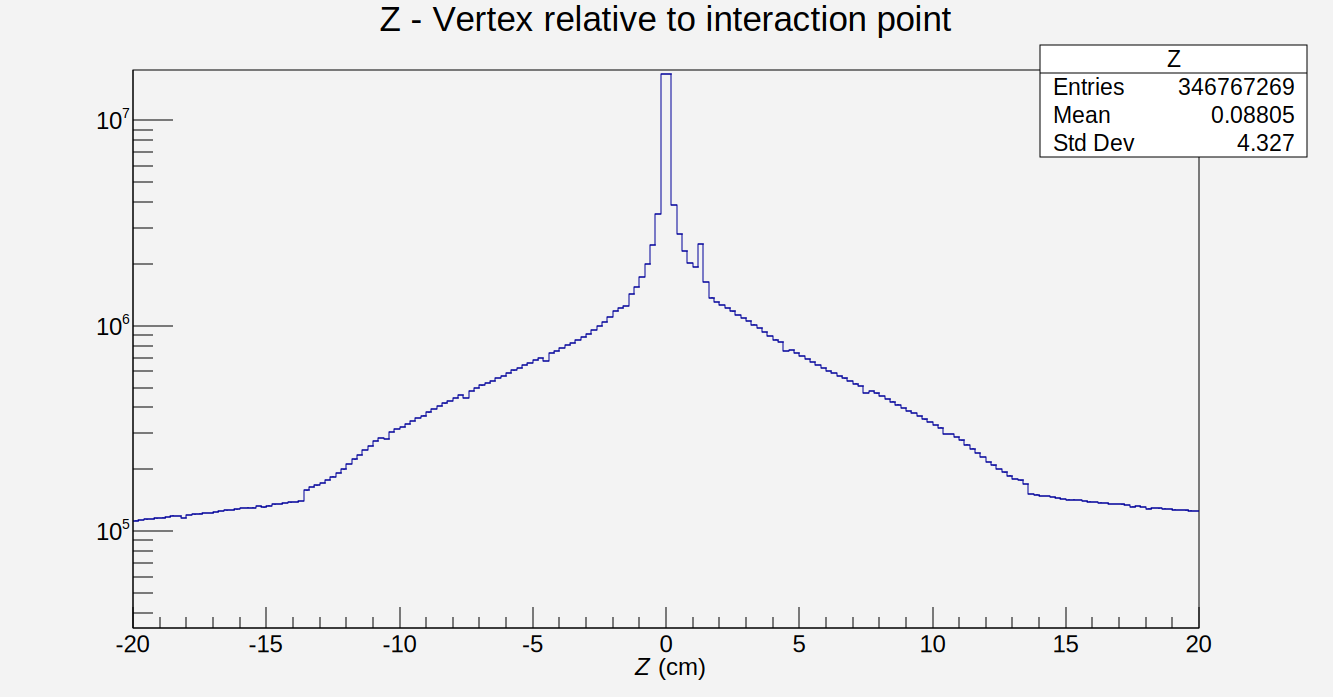
\includegraphics[width=\linewidth]{Plots/pass4_TracksIU/Z.pdf}
        \caption{Histogram of the $z$-position of the collision vertex. A gaussian function is fit to the data, with $\mu=0.2951$, $\sigma=6.0205$. Note that this is not the position as determined by the ITS alone as that information is not in the data model at present. Each entry is a collision, not a track.}
        \label{fig:ITS_Z}
    \end{subfigure}
\caption[Histograms of $\eta$, $\varphi$, \OldTexttt{nClusters}, and $z$ for tracks in the ITS]{Histograms of kinematic variables of tracks detected by the ITS as well as of collisions.}
\label{fig:ITS_1D}
\end{figure}

The $\varphi$ distribution in \cref{fig:ITS_phi} looks much more uniform, at least on the whole, than in \cref{fig:nohasITS_phi}. This is made more obvious when taking \cref{fig:nohasITS_phi_no_ITS} into account as there appears to be no pattern or symmetry in the $\varphi$ distribution of tracks when not detected in the ITS. No reason for this is apparent to us so this requires a more in-depth investigation. The valley in \cref{fig:ITS_phi} at about 4.3, and smaller ones in other places, is certainly a concern. \Cref{fig:ITS_eta_phi} helps to elucidate the situation as we can see there is no $\eta$ dependence on the large gap, so we are inclined to say that a whole strip of detectors in the ITS, running along the $z$-axis, was not functioning properly. This is reasonable as the electronics in the ITS run in that direction, grouping pixel chips together. 

Other smaller gaps can also be seen, spanning short ranges of $\eta$, which would imply short strips of pixel chips weren't working properly.

\begin{figure}[h]
    \begin{center}
        \includegraphics[width=.8\textwidth]{Plots/pass4_TracksIU/eta_phi.pdf}
        \caption[$\eta$-$\varphi$ histogram for tracks in the ITS]{Histogram of $\eta$ and $\varphi$ for tracks detected in the ITS. The valley at $\varphi\approx 4.3$ can clearly be seen, with no specific $\eta$ region being affected. Note a few other smaller strips of lower counts.}
        \label{fig:ITS_eta_phi}
    \end{center}
\end{figure}

Looking at \cref{fig:ITS_NCls_InnerBarrel} in comparison to \cref{fig:nohasITS_NCls_InnerBarrel}, we see a decrease in the number of tracks with no clusters in the inner barrel. This is clearly as expected. Lastly, the $z$-position of the collision vertex is shown in \cref{fig:ITS_Z} with a gaussian function fit to it. Important to note here is that each entry in the histogram is not a track, as it has been before, but rather a collision in the \texttt{aod::Collisions} table. This is less of an indicator of the performance of the ITS but is always a useful plot to look at to make sure that collisions are happening both as close to the IP as possible but also symmetrically around the IP. Both these conditions are met in this case, within acceptable tolerance. 

\bigskip

The last histograms to interrogate are ones corresponding to the clusters contributing to tracks in the ITS, shown in \cref{fig:ITS_Clusters}. The left is easy to interpret, showing the number of ITS clusters used in each track. Interestingly it appears to have a minimum of 4 clusters per track. If these tracks are from the TPC regime, this doesn't make sense, but if they are standalone tracks then we may have discovered something about the method used.

\begin{figure}[h]%
    \centering
    \begin{subfigure}[t]{.49\linewidth}
        \centering
        \includegraphics[width=\linewidth]{Plots/pass4_TracksIU/itsNCls.pdf}
        \caption{Histogram of number of clusters in the entire ITS that contribute to a given track. Note the cut-off at 4, seeming to imply a minimum number of clusters per track.}
        \label{fig:ITS_NCls}
    \end{subfigure}
    \hfill
    \begin{subfigure}[t]{.49\linewidth}
        \centering
        \includegraphics[width=\linewidth]{Plots/pass4_TracksIU/itsClusterMap.pdf}
        \caption{Histogram of the so-called ``Cluster Map'' of the ITS, where each layer in the ITS is assigned a bit, starting from the innermost.}
        \label{fig:ITS_ClusterMap}
    \end{subfigure}
\caption[Histograms of cluster information for tracks in the ITS]{Additional histograms with information about the ITS clusters used in track finding.}
\label{fig:ITS_Clusters}
\end{figure}

On the right of \cref{fig:ITS_Clusters} is the ``Cluster Map'' of the ITS. The column in the data model contains an 8 bit unsigned integer with each bit assigned to a layer, excluding the last bit. If a track has a cluster in a specific layer, the bit is set to 1, otherwise it is set to 0. Since integers have unique representations in binary, we can see exactly which layers contributed to a given track simply by decoding the integer. As seen in \cref{fig:ITS_ClusterMap}, the lowest is 15 meaning the innermost 4 layers had clusters contributing, and the highest is 127 meaning all layers had clusters contributing. In between those is all combinations of the 7 bits, but only those with 4 or more clusters, as expected from \cref{fig:ITS_NCls}. 